% LuaLaTeX

\documentclass[a4paper, twoside, 12pt]{article}
\usepackage[latin]{babel}
%\usepackage[landscape, left=3cm, right=1.5cm, top=2cm, bottom=1cm]{geometry} % okraje stranky
\usepackage[landscape, a4paper, mag=1166, truedimen, left=2cm, right=1.5cm, top=1.6cm, bottom=0.95cm]{geometry} % okraje stranky

\usepackage{fontspec}
\setmainfont[FeatureFile={junicode.fea}, Ligatures={Common, TeX}, RawFeature=+fixi]{Junicode}
%\setmainfont{Junicode}

% shortcut for Junicode without ligatures (for the Czech texts)
\newfontfamily\nlfont[FeatureFile={junicode.fea}, Ligatures={Common, TeX}, RawFeature=+fixi]{Junicode}

\usepackage{multicol}
\usepackage{color}
\usepackage{lettrine}
\usepackage{fancyhdr}

% usual packages loading:
\usepackage{luatextra}
\usepackage{graphicx} % support the \includegraphics command and options
\usepackage{gregoriotex} % for gregorio score inclusion
\usepackage{gregoriosyms}
\usepackage{wrapfig} % figures wrapped by the text
\usepackage{parcolumns}
\usepackage[contents={},opacity=1,scale=1,color=black]{background}
\usepackage{tikzpagenodes}
\usepackage{calc}
\usepackage{longtable}
\usetikzlibrary{calc}

\setlength{\headheight}{14.5pt}

% Commands used to produce a typical "Conventus" booklet

\newenvironment{titulusOfficii}{\begin{center}}{\end{center}}
\newcommand{\dies}[1]{#1

}
\newcommand{\nomenFesti}[1]{\textbf{\Large #1}

}
\newcommand{\celebratio}[1]{#1

}

\newcommand{\hora}[1]{%
\vspace{0.5cm}{\large \textbf{#1}}

\fancyhead[LE]{\thepage\ / #1}
\fancyhead[RO]{#1 / \thepage}
\addcontentsline{toc}{subsection}{#1}
}

% larger unit than a hora
\newcommand{\divisio}[1]{%
\begin{center}
{\Large \textsc{#1}}
\end{center}
\fancyhead[CO,CE]{#1}
\addcontentsline{toc}{section}{#1}
}

% a part of a hora, larger than pars
\newcommand{\subhora}[1]{
\begin{center}
{\large \textit{#1}}
\end{center}
%\fancyhead[CO,CE]{#1}
\addcontentsline{toc}{subsubsection}{#1}
}

% rubricated inline text
\newcommand{\rubricatum}[1]{\textit{#1}}

% standalone rubric
\newcommand{\rubrica}[1]{\vspace{3mm}\rubricatum{#1}}

\newcommand{\notitia}[1]{\textcolor{red}{#1}}

\newcommand{\scriptura}[1]{\hfill \small\textit{#1}}

\newcommand{\translatioCantus}[1]{\vspace{1mm}%
{\noindent\footnotesize \nlfont{#1}}}

% pruznejsi varianta nasledujiciho - umoznuje nastavit sirku sloupce
% s prekladem
\newcommand{\psalmusEtTranslatioB}[3]{
  \vspace{0.5cm}
  \begin{parcolumns}[colwidths={2=#3}, nofirstindent=true]{2}
    \colchunk{
      \input{#1}
    }

    \colchunk{
      \vspace{-0.5cm}
      {\footnotesize \nlfont
        \input{#2}
      }
    }
  \end{parcolumns}
}

\newcommand{\psalmusEtTranslatio}[2]{
  \psalmusEtTranslatioB{#1}{#2}{8.5cm}
}


\newcommand{\canticumMagnificatEtTranslatio}[1]{
  \psalmusEtTranslatioB{#1}{temporalia/extra-adventum-vespers/magnificat-boh.tex}{12cm}
}
\newcommand{\canticumBenedictusEtTranslatio}[1]{
  \psalmusEtTranslatioB{#1}{temporalia/extra-adventum-laudes/benedictus-boh.tex}{10.5cm}
}

% volne misto nad antifonami, kam si zpevaci dokresli neumy
\newcommand{\hicSuntNeumae}{\vspace{0.5cm}}

% prepinani mista mezi notovymi osnovami: pro neumovane a neneumovane zpevy
\newcommand{\cantusCumNeumis}{
  \setgrefactor{17}
  \global\advance\grespaceabovelines by 5mm%
}
\newcommand{\cantusSineNeumas}{
  \setgrefactor{17}
  \global\advance\grespaceabovelines by -5mm%
}

% znaky k umisteni nad inicialu zpevu
\newcommand{\superInitialam}[1]{\gresetfirstlineaboveinitial{\small {\textbf{#1}}}{\small {\textbf{#1}}}}

% pars officii, i.e. "oratio", ...
\newcommand{\pars}[1]{\textbf{#1}}

\newenvironment{psalmus}{
  \setlength{\parindent}{0pt}
  \setlength{\parskip}{5pt}
}{
  \setlength{\parindent}{10pt}
  \setlength{\parskip}{10pt}
}

%%%% Prejmenovat na latinske:
\newcommand{\nadpisZalmu}[1]{
  \hspace{2cm}\textbf{#1}\vspace{2mm}%
  \nopagebreak%

}

% mode, score, translation
\newcommand{\antiphona}[3]{%
\hicSuntNeumae
\superInitialam{#1}
\includescore{#2}

#3
}
 % Often used macros
%%%% Preklady jednotlivych zpevu (nektere se opakuji, a je dobre mit je
% vsechny na jedne hromade)

\newcommand{\trOratioAnteOfficium}{\translatioCantus{Otevři, Pane, má ústa, abych chválil tvé svaté jméno.
Očisti mé srdce od všech marnivých, zvrácených a~jiných myšlenek, osvěť rozum, rozněť cit,
abych mohl důstojně, soustředěně a~zbožně recitovat a~vysloužil si být
vyslyšen před tváří tvé velebnosti. Skrze Krista…}}

\newcommand{\trOratioPostOfficium}{\translatioCantus{\textit{Následující modlitbu
opatřil pro ty, kdo ji zbožně vyřknou po hodinkách, zesnulý papež Lev X.
odpustky za hříchy vzniklé při konání hodinek z~lidské křehkosti. Říká se
vkleče.}
Svatosvaté a~nerozdílné Trojici, ukřižovanému lidství našeho Pána Ježíše
Krista, přeblažené a~přeslavné plodné neporušenosti vždy Panny Marie
i~souhrnu všech svatých buď ode všeho stvoření věčná chvála, čest a~sláva, nám
pak buď dáno odpuštění všech hříchů, po nekonečné věky věků. Amen.}}

% HOURS ---

\newcommand{\trAntI}{\translatioCantus{Jasné narození slavné Panny Marie,
z pokolení (dosl. ze semene) Abrahámova, vzešlé z kmene Judova, z rodu Davidova.}}
\newcommand{\trAntII}{\translatioCantus{Dnes je Narození svaté Panny 
Marie, jejíž předrahý život osvěcuje všechny církve.}}

\newcommand{\trAntIII}{\translatioCantus{Maria, jež vzešla 
z královského rodu, září; myslí i duchem ji zbožně prosíme, aby 
nám pomáhala svými přímluvami.}}

\newcommand{\trAntIV}{\translatioCantus{Srdcem i duchem pějme Kristu 
k slávě o této svaté slavnosti vznešené Rodičky Boží Marie.}}

\newcommand{\trAntV}{\translatioCantus{Příjemně \notitia{?} 
oslavujme Narození blahoslavené Marie,
aby se ona za nás přimlouvala u Pána Ježíše Krista.}}

\newcommand{\trCapituli}{\translatioCantus{Před věky, na počátku mě stvořil, potrvám věčně. Ve svatém Stanu jsem před ním konala službu.}}

\newcommand{\trRespVesp}{\translatioCantus{Buď zdráva, Maria,
plná milosti: \grestar{} Pán s tebou. \Vbardot{} Požehnaná jsi mezi ženami,
a požehnaný plod života (ve smyslu lůna, břicha) tvého.}}

\newcommand{\trVersus}{\translatioCantus{\Vbardot{} Dnes je Narození svaté Panny Marie. \Rbardot{} Jejíž předrahý život osvěcuje všechny církve.}}

\newcommand{\trAntMagnificatI}{\translatioCantus{Konejme památku
veledůstojného narození slavné Panny Marie,
jíž se dostalo mateřské důstojnosti bez ztráty panenské cudnosti.}}

% Tento preklad je vice nez nejisty a ani alternativy, ktere jsem
% videl, me nepresvedcily...
\newcommand{\trAntBenedictus}{\translatioCantus{Slavnostně slavme 
dnešní narození Marie, vždy Panny a Rodičky Boží: v něm se objevuje
vysokost trůnu (totiž Marie, trůnu Božího Syna), aleluja.}}

\newcommand{\trAntMagnificatII}{\translatioCantus{Tvé narození,
Bohorodičko Panno, vyhlásilo radost celému světu:
z tebe totiž vzešlo Slunce spravedlnosti, Kristus, náš Bůh:
jenž zrušil kletbu a dal nám požehnání: přemohl smrt a dal nám život věčný.}}

\newcommand{\trOrationis}{\translatioCantus{Prosíme tě, Bože, 
uděl svým služebníkům dar nebeské milosti,
aby těm, jimž slehnutím blahoslavené Panny vyvstal počátek spásy, 
slavnost k poctě jejího narození přinesla
rozhojnění pokoje.
Skrze tvého Syna, našeho Pána Ježíše Krista, který s tebou žije a kraluje,
Bůh, v jednotě Ducha svatého po všechny věky věků.}}

\newcommand{\trFideliumAnimae}{\translatioCantus{\Vbardot{} Duše věrných ať pro
milosrdenství Boží odpočívají v~pokoji. \Rbardot{} Amen.}}

% Completorium

\newcommand{\trJubeDomne}{\translatioCantus{Rač, pane, požehnat.}}

\newcommand{\trComplBenedictio}{\translatioCantus{Pokojnou noc a~svatou smrt
nechť nám dopřeje všemohoucí Pán. \Rbardot{} Amen.}}

\newcommand{\trComplLectioBr}{\translatioCantus{Buďte střízliví, bděte.
Váš protivník Ďábel obchází jako lev řvoucí a~hledá, koho by pohltil.
Postavte se proti němu pevní ve víře.  Ale ty, Pane, smiluj se nad námi.
\Rbardot{} Bohu díky.}}

\newcommand{\trComplAntI}{\translatioCantus{Rač se smilovati nade mnou,
Hospodine, a vyslyš mou modlitbu.}}

\newcommand{\trComplCapituli}{\translatioCantus{Jsi přece, Hospodine,
uprostřed nás a~jmenujeme se po tobě.  Neopouštěj nás, Pane, náš Bože.}}

\newcommand{\trRespCompl}{\translatioCantus{Do tvých rukou, Pane, \grestar{}
poroučím svého ducha. \Vbardot{} Ty mne zachráníš, Pane, Bože věrný.}}

\newcommand{\trComplVersus}{\translatioCantus{\Vbardot{} Střez mne jako zřítelnici oka,
aleluja. \Rbardot{} Ve stínu svých křídel uschovej mne, aleluja.}}

\newcommand{\trAntSalvaNos}{\translatioCantus{Ochraňuj nás, Pane, když
bdíme, a~buď s~námi, když spíme, ať bdíme s~Kristem a~odpočíváme v~pokoji.}}

\newcommand{\trComplOrationis}{\translatioCantus{Zavítej, prosíme, Pane, sem
do našeho příbytku a~daleko od něj zažeň všechny úklady nepřítele. Ať tu
bydlí tví svatí andělé a~tvoje požehnání buď nad ním stále. Skrze…}}

\newcommand{\trSalveRegina}{\translatioCantus{Zdrávas Královno, matko
milosrdenství, živote, sladkosti a naděje naše, buď zdráva!
K tobě voláme, vyhnaní synové Evy,
k tobě vzdycháme, lkajíce a plačíce
v tomto slzavém údolí.
A proto, orodovnice naše,
obrať k nám své milosrdné oči
a Ježíše, požehnaný plod života svého,
nám po tomto putování ukaž,
ó milostivá, ó přívětivá,
ó přesladká, Panno Maria!}}

\newcommand{\trOraProNobis}{\translatioCantus{\Vbardot{} 
Oroduj za nás, svatá Boží Rodičko,
\Rbardot{} aby nám Kristus dal účast na svých zaslíbeních.}}

% Matutinum

\newcommand{\trMatInvitatorium}{\translatioCantus{}}

\newcommand{\trMatVeniteA}{\translatioCantus{Pojďte, chvalme s~radostí Pána,
s~jásotem slavme Boha, svou spásu; předstupme před tvář jeho s~díky, písně plesu pějme jemu.}}

\newcommand{\trMatVeniteB}{\translatioCantus{Neboť Bůh veliký jest Hospodin, a~král nade všecky bohy.
Jsouť v~jeho ruce všecky hlubiny země, temena hor jsou majetek jeho.}}

\newcommand{\trMatVeniteC}{\translatioCantus{Jehoť jest moře, neb on je učinil; i~souš
je dílo jeho rukou. Pojďme, klanějme se, padněme, klekněme před Pánem, svým
tvůrcem. Jeť on Pán, náš Bůh, a~my jsme lid, jejž on vodí a~ovce, jež pase.}}

\newcommand{\trMatVeniteD}{\translatioCantus{Kéž byste poslechli dnes hlasu jeho:
,,Nezatvrzujte svých srdcí jak v~Hádce, jak v~Pokušení na poušti, kde vaši otcové pokoušeli mne,
zkoušeli mne, ač vídali skutky mé.``}}

\newcommand{\trMatVeniteE}{\translatioCantus{Čtyřicet roků mrzel jsem se na to pokolení
a~řekl jsem: ,,Lid je to myslí stále bloudící``! Oni však nechtěli znáti mé cesty, takže jsem
přisáhl ve svém hněvu: ,,Nedojdou odpočinku mého!\mbox{}``}}

\newcommand{\trMatAntI}{\translatioCantus{}}

\newcommand{\trMatAntII}{\translatioCantus{}}

\newcommand{\trMatAntIII}{\translatioCantus{}}

\newcommand{\trMatVersusI}{\translatioCantus{}}

\newcommand{\trMatAbsolutioI}{\translatioCantus{Vyslyš Pane Ježíši Kriste
prosby svých služebníků \gredagger{} a~smiluj se nad námi, \grestar{} jenž
s~Otcem a~Duchem…}}

\newcommand{\trMatBenedictioI}{\translatioCantus{Rač, pane, požehnat.
Věčný Otec nám stále žehnej. \Rbardot{} Amen.}}

\newcommand{\trMatLecI}{\translatioCantus{Kéž by mě zulíbal polibky svých úst. 
Tvé milování je nad víno lahodnější;
vybraně voní tvé voňavky;
rozlévající se olej je tvé jméno,
proto tě dívky milují.
Strhni mě za sebou, poběžme!
Král mě uvedl do svých komnat;
budeš nám radostí a jásotem.
Víc než víno oslavíme tvé milování;
věru po právu jsi milován!
Snědá jsem, a přece krásná, jeruzalémské dcery,
jako stany kedarské,
jako šalmské závěsy.
}}

\newcommand{\trMatRespI}{\translatioCantus{}}

\newcommand{\trMatBenedictioII}{\translatioCantus{Rač, pane, požehnat.
Jednorozený Boží Syn nám žehnej \grestar{} a nám pomáhej. \Rbardot{} Amen.}}

\newcommand{\trMatLecII}{\translatioCantus{Nehleďte na mou osmahlou pleť:
to mě slunce ožehlo.
Synové mé matky se na mne rozzlobili,
poslali mě hlídat vinice.
A svou vinici, tu jsem nehlídala!
Pověz mi tedy, ty, jehož miluje mé srdce:
kam zavedeš své stádo pást,
kde ho necháš za poledne odpočívat?
Abych už nebloudila jako tulačka
poblíž stád druhů tvých.
Nevíš-li to, nejrásnější z žen,
jdi po stopách stáda
a kůzlata svá zaveď, ať se pasou
poblíž obydlí pastýřů.
Ke své klisně zapřažené do vozu faraonova
tebe, mé milá, přirovnávám.
Stále krásné jsou tvé líce s náušnicemi
i tvé hrdlo v náhrdelnících.}}

\newcommand{\trMatRespII}{\translatioCantus{}}

\newcommand{\trMatBenedictioIII}{\translatioCantus{Rač, pane, požehnat.
Milost Ducha Svatého ať osvítí nám smysly \grestar{} i srdce. \Rbardot{} Amen.}}

\newcommand{\trMatLecIII}{\translatioCantus{Zhotovíme ti zlaté náušnice
a kuličky ze stříbra.
Když král stoluje,
vydechuje můj nard svou vůni.
Můj milý je polštářek s myrhou,
jenž mi odpočívá mezi ňadry.
Můj milý je hrozen šáchoru
ve vinicích v Engadi.
Jak jsi krásná, milá moje,
jak jsi krásná!
Tvé oči jsou holubice.
Jak jsi krásný, můj milý,
jak líbezný!
Naše lože je samá zeleň.
Trámoví našeho domu je z cedru,
naše ostění z cypřiše.}}

\newcommand{\trMatRespIII}{\translatioCantus{}}

\newcommand{\trMatAntIV}{\translatioCantus{}}

\newcommand{\trMatAntV}{\translatioCantus{}}

\newcommand{\trMatAntVI}{\translatioCantus{}}

\newcommand{\trMatVersusII}{\translatioCantus{}}

\newcommand{\trMatAbsolutioII}{\translatioCantus{
Tvá milost a laskavost nechť nám pomáhá, jenž žiješ a vládneš s Otcem a Svatým Duchem na věky věků.}}

\newcommand{\trMatBenedictioIV}{\translatioCantus{Rač, pane, požehnat.
Bůh Otec všemohoucí, \grestar{} buď k nám milostivý a odpouštějící. \Rbardot{} Amen.}}

\newcommand{\trMatLecIV}{\translatioCantus{}}

\newcommand{\trMatRespIV}{\translatioCantus{}}

\newcommand{\trMatBenedictioV}{\translatioCantus{}}

\newcommand{\trMatLecV}{\translatioCantus{}}

\newcommand{\trMatRespV}{\translatioCantus{}}

\newcommand{\trMatBenedictioVI}{\translatioCantus{Rač, pane, požehnat.
Bůh rozněť v nás oheň své lásky. \Rbardot{} Amen.}}

\newcommand{\trMatLecVI}{\translatioCantus{}}

\newcommand{\trMatRespVI}{\translatioCantus{}}

\newcommand{\trMatAntVII}{\translatioCantus{}}

\newcommand{\trMatAntVIII}{\translatioCantus{}}

\newcommand{\trMatAntIX}{\translatioCantus{}}

\newcommand{\trMatVersusIII}{\translatioCantus{}}

\newcommand{\trMatAbsolutioIII}{\translatioCantus{Z okovů našich hříchů,
\grestar{} vysvoboď nás všemohoucí a milosrdný Pán. \Rbardot{} Amen.}}

\newcommand{\trMatBenedictioVII}{\translatioCantus{Rač, pane, požehnat.
Čtení evangelia nechť je nám \grestar{} spásou a ochranou. \Rbardot{} Amen.}}

\newcommand{\trMatLecVIIa}{\translatioCantus{
  Rodokmen Ježíše Krista, syna Davidova, syna Abrahámova:
  Abrahám zplodil Izáka,
  Izák zplodil Jakuba.}}

\newcommand{\trMatLecVIIb}{\translatioCantus{}}

\newcommand{\trMatRespVII}{\translatioCantus{}}

\newcommand{\trMatBenedictioVIII}{\translatioCantus{Rač, pane, požehnat.
\Rbardot{} Amen.}}

\newcommand{\trMatLecVIII}{\translatioCantus{}}

\newcommand{\trMatRespVIII}{\translatioCantus{}}

\newcommand{\trMatBenedictioIX}{\translatioCantus{Rač, pane, požehnat.
Do společnosti občanů nebes \grestar{} ať nás dovede král andělů.
\Rbardot{} Amen.}}

\newcommand{\trMatLecIX}{\translatioCantus{}}

% from the Czech Liturgia horarum
\newcommand{\trTeDeum}{\begin{translatioMulticol}{3}

Bože, tebe chválíme, 
tebe, Pane, velebíme.

Tebe, věčný Otče, 
oslavuje celá země.

Všichni andělé, 
cherubové i~serafové,

všechny mocné nebeské zástupy 
bez ustání volají:

Svatý, Svatý, Svatý, 
Pán, Bůh zástupů.

Plná jsou nebesa i~země 
tvé vznešené slávy.

Oslavuje tě 
sbor tvých apoštolů,

chválí tě 
velký počet proroků,

vydává o~tobě svědectví 
zástup mučedníků;

a~po celém světě 
vyznává tě tvá církev:

neskonale velebný, 
všemohoucí Otče,

úctyhodný Synu Boží, 
pravý a~jediný,

božský Utěšiteli, 
Duchu svatý.

Kriste, Králi slávy, 
tys od věků Syn Boha Otce;

abys člověka vykoupil, 
stal ses člověkem a~narodil ses z~Panny;

zlomil jsi osten smrti 
a~otevřel věřícím nebe;

sedíš po Otcově pravici 
a~máš účast na jeho slávě.

Věříme, že přijdeš soudit, 

a~proto tě prosíme:
přispěj na pomoc svým služebníkům, 
vždyť jsi je vykoupil svou předrahou krví;

dej, ať se radují s~tvými svatými 
ve věčné slávě.

Zachraň, Pane, svůj lid, žehnej svému dědictví, 
veď ho a~stále pozvedej.

Každý den tě budeme velebit 
a~chválit tvé jméno po všechny věky.

Pomáhej nám i~dnes, 
ať se nedostaneme do područí hříchu.

Smiluj se nad námi, Pane, 
smiluj se nad námi.

Ať spočine na nás tvé milosrdenství, 
jak doufáme v~tebe.

Pane, k~tobě se utíkáme, 
ať nejsme zahanbeni na věky. 
\end{translatioMulticol}}

\newcommand{\trMatEvangelium}{\translatioCantus{
  Rodokmen Ježíše Krista, syna Davidova, syna Abrahámova:
  Abrahám zplodil Izáka,
  Izák zplodil Jakuba,
  Jakub zplodil Judu a jeho bratry,
  Juda zplodil Farese a Zaru z Tamary,
  Fares zplodil Esroma,
  Esrom zplodil Arama,
  Aram zplodil Aminadaba,
  Aminadab zplodil Naasona,
  Naason zplodil Salmona,
  Salmon zplodil Boaze z Rahaby,
  Boaz zplodil Jobeda z Rut,
  Jobed zplodil Jessea,
  Jesse zplodil krále Davida.
  David zplodil Šalomouna z Uriášovy ženy,
  Šalomoun zplodil Roboama,
  Roboam zplodil Abiu,
  Abia zplodil Asu,
  Asa zplodil Josafata,
  Josafat zplodil Jorama,
  Joram zplodil Oziáše,
  Oziáš zplodil Joatama,
  Joatam zplodil Achaze,
  Achaz zplodil Ezechiáše,
  Ezechiáš zplodil Manasesa,
  Manases zplodil Amona,
  Amon zplodil Josiáše,
  Josiáš zplodil Jechoniáše a jeho bratry;
  tehdy došlo k odvlečení do Babylonu.
  Po odvlečení do Babylonu:
  Jechoniáš zplodil Salatiela,
  Salatiel zplodil Zorobabela,
  Zorobabel zplodil Abiuda,
  Abiud zplodil Eljakima,
  Eljakim zplodil Azora,
  Ator zplodil Sadoka,
  Sadok zplodil Achima,
  Achim zplodil Eliuda,
  Eliud zplodil Eleazara,
  Eleatar zplodil Matana,
  Matan zplodil Jakuba,
  Jakub zplodil Josefa, manžela Marie,
  z níž se narodil Ježíš, který se nazývá Kristus.}}

\newcommand{\trTeDecetLaus}{\translatioCantus{Tobě chvála, Tobě zpěvy, Tobě
sláva, Bohu Otci i~Synu i~Svatému Duchu, na věky věků. \Rbardot{} Amen.}}

% MASS ---

\newcommand{\trIntroitus}{\translatioCantus{Radujme se všichni
v Pánu, slavíce svátek ke cti Panny Marie: z něj se radují andělé
a spoluchválí Božího Syna. \textit{\color{red}Žl.} Má ústa vydala dobré slovo,
přednáším svá díla králi.}}

\newcommand{\trGraduale}{\translatioCantus{Požehnaná a ctihodná jsi,
Panno Maria: nedotčená (co do panenství) jsi byla shledána matkou
Spasitele. \Vbardot{} Panno Boží Rodičko, ten, jehož nepojme ani celý svět,
se uzavřel do tvých útrob, když se stal člověkem.}}

\newcommand{\trAlleluia}{\translatioCantus{Aleluja. \Vbardot{} Skvělá slavnost
slavné Panny Marie, z pokolení (dosl. ze semene) Abrahámova, vzešlé z kmene 
Judova, z rodu Davidova.}}

\newcommand{\trOffertorium}{\translatioCantus{Blažená jsi, Panno Maria,
tys nosila Stvořitele všeho; porodila jsi toho, který tě utvořil,
a na věky zůstáváš Pannou.}}

\newcommand{\trCommunio}{\translatioCantus{Budou mě blahoslavit
všechna pokolení, protože mi učinil veliké věci ten, který je mocný.}}

% LITTLE HOURS ---

\newcommand{\trVersusTertia}{\translatioCantus{\Vbardot{} \Rbardot{}}}

\newcommand{\trCapituliEtSic}{\translatioCantus{
Tak jsem se usadila na Sionu a v milovaném městě jsem nalezla odpočinek,
v Jeruzalémě vykonávám svou moc.
Zakořenila jsem u lidu plného slývy, na panství Páně, v jeho dědictví.}}

\newcommand{\trVersusSexta}{\translatioCantus{\Vbardot{} \Rbardot{}}}

\newcommand{\trCapituliInPlateis}{\translatioCantus{
Na planině jako skořicovník a akant jsem vydávala vůni, jako vybraná myrha
jsem voněla.}}

\newcommand{\trVersusNona}{\translatioCantus{\Vbardot{} \Rbardot{}}}
 % Czech translations of the proper texts

\newcommand{\annusEditionis}{2017}

%%%% Vicekrat opakovane kousky

\newcommand{\anteOrationem}{
  \rubrica{Ante Orationem, cantatur a Superiore:}

  \pars{Supplicatio Litaniæ.}

  \cuminitiali{}{temporalia/supplicatiolitaniae.gtex}

  \pars{Oratio Dominica.}

  \cuminitiali{}{temporalia/oratiodominica.gtex}

  \rubrica{Deinde dicitur ab Hebdomadario:}

  \cuminitiali{}{temporalia/dominusvobiscum-solemnis.gtex}

  \rubrica{In choro monialium loco Dominus vobiscum dicitur:}

  \sineinitiali{temporalia/domineexaudi.gtex}
}

\setlength{\columnsep}{30pt} % prostor mezi sloupci

%%%%%%%%%%%%%%%%%%%%%%%%%%%%%%%%%%%%%%%%%%%%%%%%%%%%%%%%%%%%%%%%%%%%%%%%%%%%%%%%%%%%%%%%%%%%%%%%%%%%%%%%%%%%%
\begin{document}

% Here we set the space around the initial.
% Please report to http://home.gna.org/gregorio/gregoriotex/details for more details and options
\grechangedim{afterinitialshift}{2.2mm}{scalable}
\grechangedim{beforeinitialshift}{2.2mm}{scalable}
\grechangedim{interwordspacetext}{0.32 cm plus 0.15 cm minus 0.05 cm}{scalable}%
\grechangedim{annotationraise}{-0.2cm}{scalable}

% Here we set the initial font. Change 38 if you want a bigger initial.
% Emit the initials in red.
\grechangestyle{initial}{\color{red}\fontsize{38}{38}\selectfont}

\pagestyle{empty}

%%%% Titulni stranka
\begin{titulusOfficii}
\nomenFesti{Dominica per Annum.}
\nomenFesti{Dominica Tempore Quadragesimæ.}
\end{titulusOfficii}

% graphic
\vspace{2.5cm}
\begin{center}
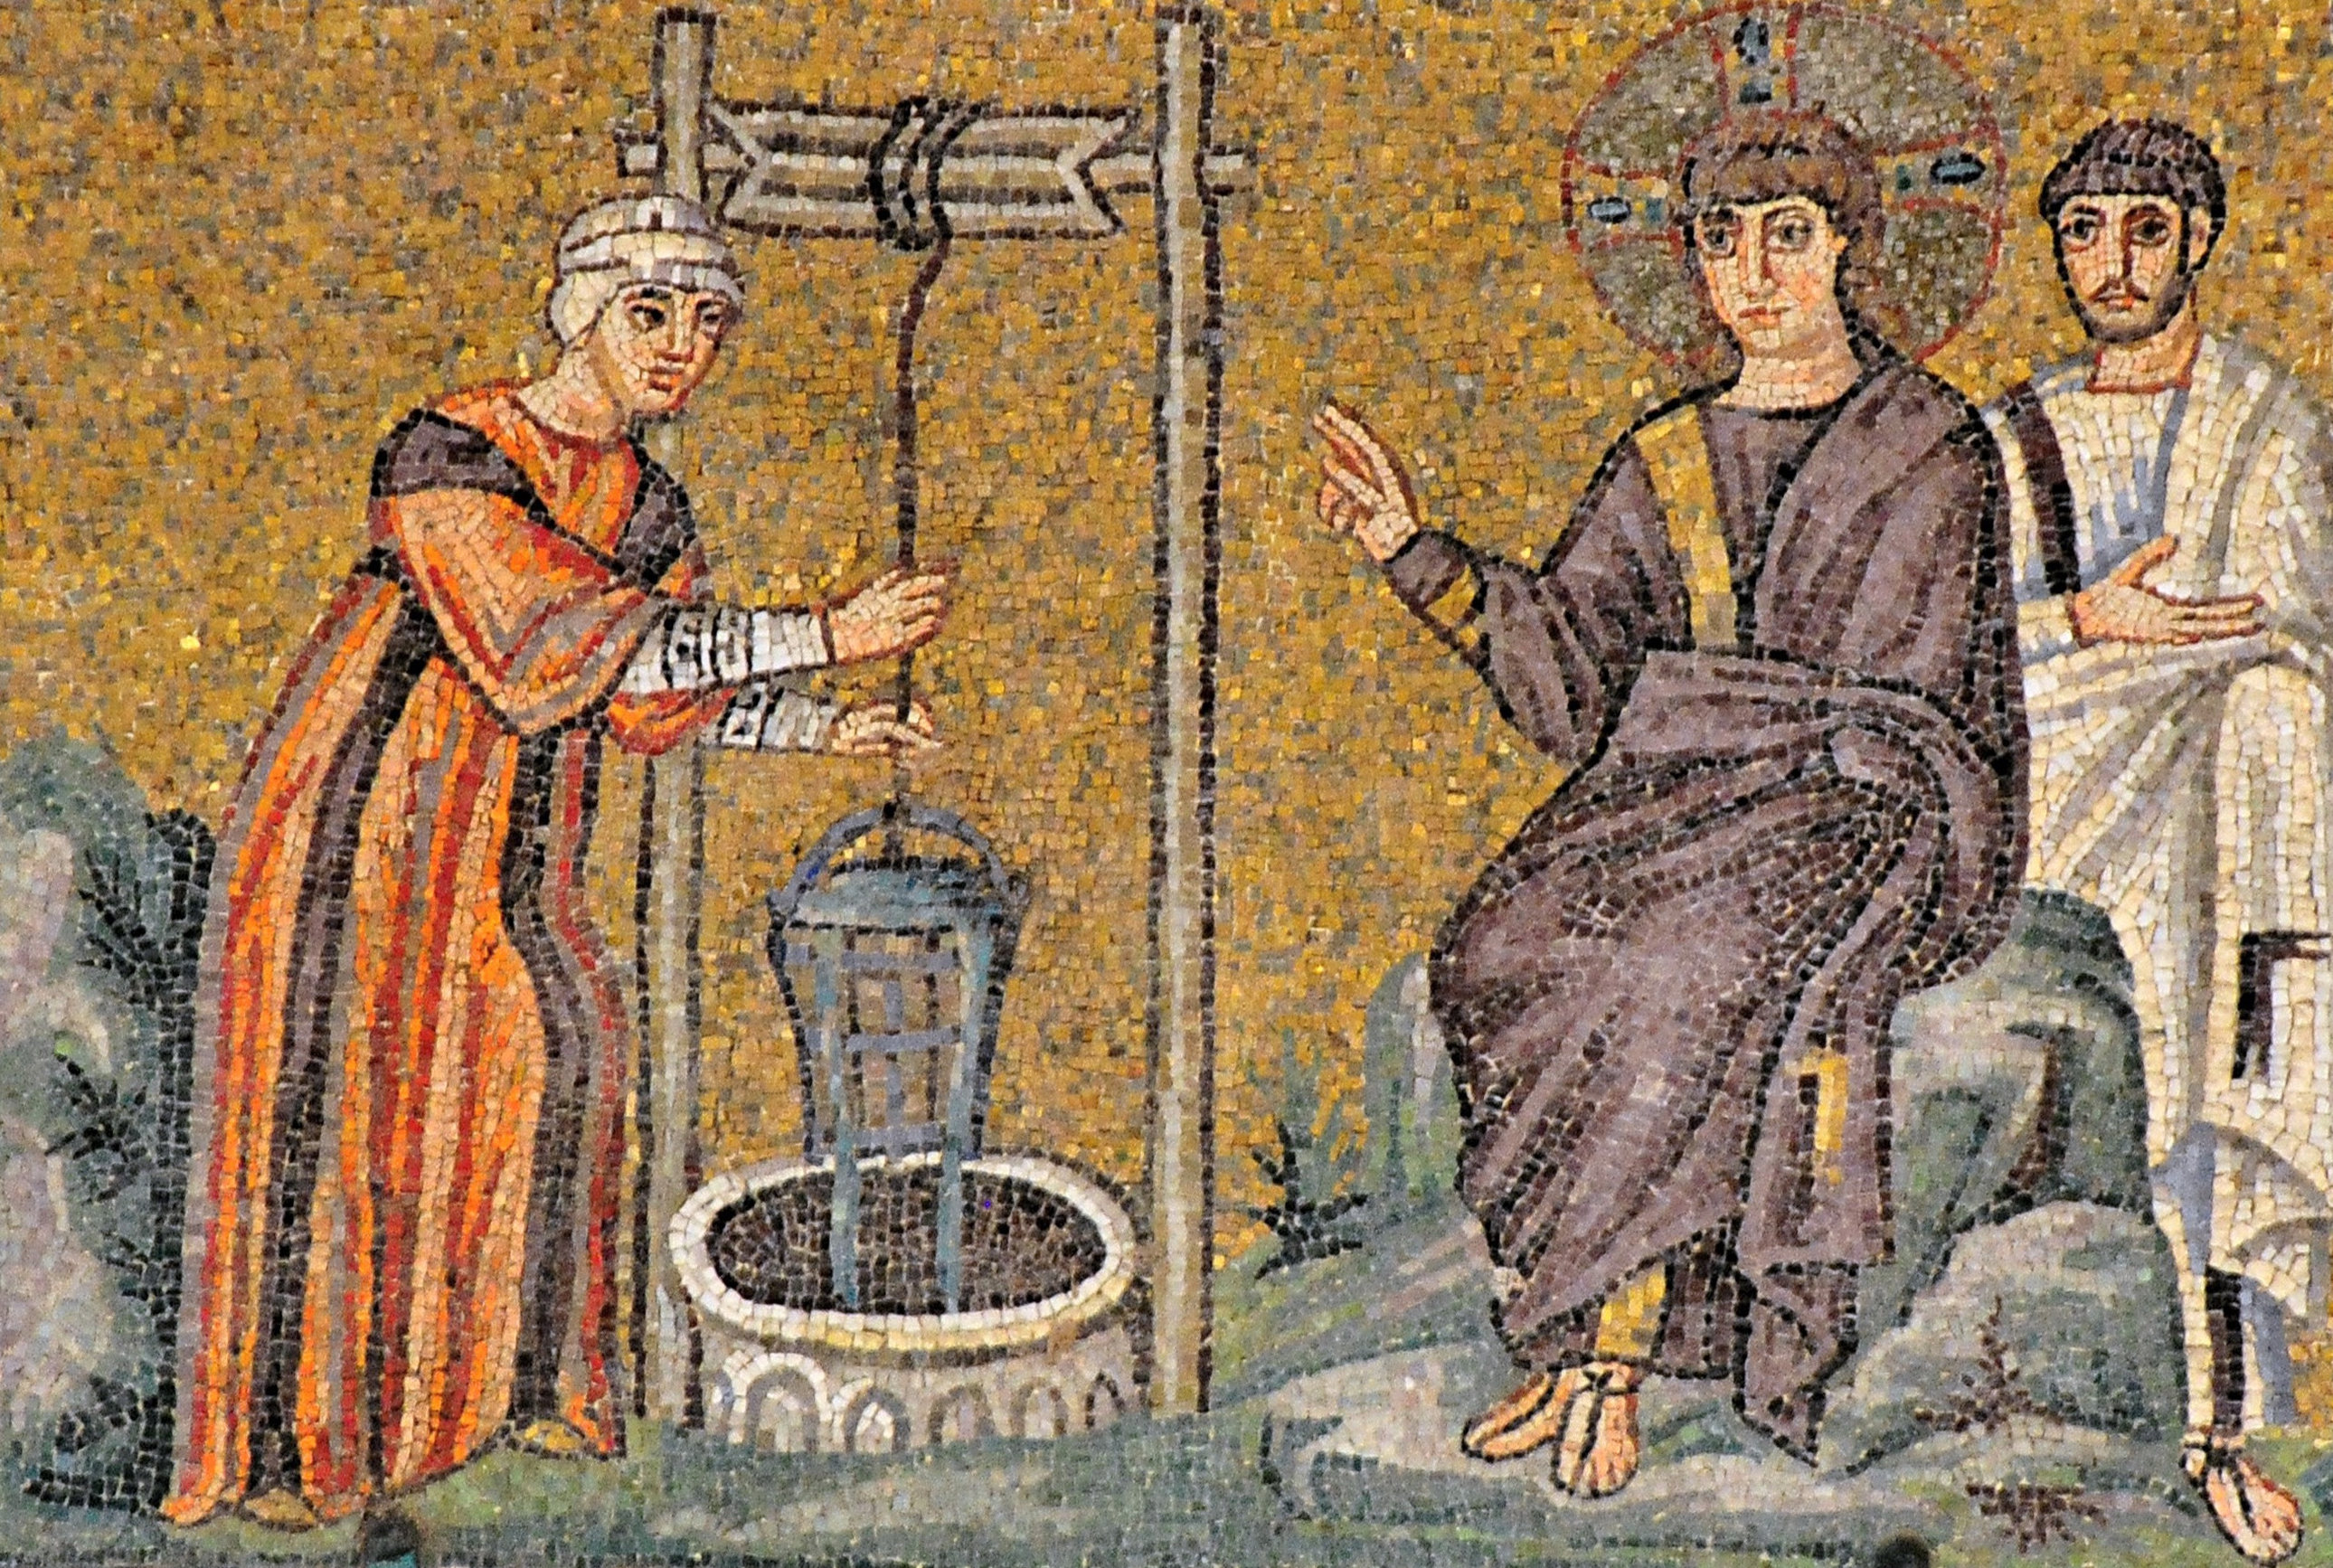
\includegraphics[width=8cm]{samaritan.jpg}
\end{center}

\vfill

\begin{center}
Ad usum et secundum consuetudines chori \guillemotright{}Conventus Choralis\guillemotleft.

Editio Sancti Wolfgangi \annusEditionis
\end{center}

\pagebreak

\renewcommand{\headrulewidth}{0pt} % no horiz. rule at the header
\fancyhf{}
\pagestyle{fancy}

\pars{Oratio ante divinum Officium.}

\lettrine{{\color{red}A}}{peri,} Dómine, os meum ad benedicéndum nomen sanctum tuum:
munda quoque cor meum ab ómnibus vanis, pervérsis, et aliénis
cogitatiónibus:
intelléctum illúmina, afféctum inflámma,
ut digne, atténte ac devóte hoc Offícium recitáre váleam,
et exaudíri mérear ante conspéctum Divínæ Maiestátis tuæ.
Per Christum, Dominum nostrum.
\Rbardot{} Amen.

Dómine, in unióne illíus divínæ intentiónis,
qua ipse in terris laudes Deo persolvísti,
has tibi Horas \rubricatum{(vel \textnormal{hanc tibi Horam})} persólvo.

\trOratioAnteOfficium

\vfill

\pars{Oratio post divinum Officium.}

\rubrica{
  Orationem sequentem devote post Officium recitantibus
  Leo Papa X. defectus, et culpas in eo persolvendo ex humana
  fragilitate contractas, indulsit, et dicitur flexis genibus.
}

\lettrine{{\color{red}S}}{acrosánctæ} et indivíduæ Trinitáti,
crucifíxi Dómini nostri Iesu Christi humanitáti,
beatíssimæ et gloriosíssimæ sempérque Vírginis Maríæ
fecúndæ integritáti, 
et ómnium Sanctórum universitáti
sit sempitérna laus, honor, virtus et glória
ab omni creatúra,
nobísque remíssio ómnium peccatórum,
per infiníta sǽcula sæculórum.
\Rbardot{} Amen.

\noindent \Vbardot{} Beáta víscera Maríæ Virginis, quæ portavérunt
ætérni Patris Fílium.\\
\Rbardot{} Et beáta úbera, quæ lactavérunt Christum Dominum.

\rubrica{Et dicitur secreto \textnormal{Pater noster.} et \textnormal{Ave María.}}

\trOratioPostOfficium

\vfill

\hora{Ad Vesperas.} %%%%%%%%%%%%%%%%%%%%%%%%%%%%%%%%%%%%%%%%%%%%%%%%%%%%%
\sideThumbs{Vesperas}

\cantusSineNeumas

\vspace{0.5cm}
\grechangedim{interwordspacetext}{0.18 cm plus 0.15 cm minus 0.05 cm}{scalable}%
\cuminitiali{}{temporalia/deusinadiutorium-alter.gtex}
\grechangedim{interwordspacetext}{0.32 cm plus 0.15 cm minus 0.05 cm}{scalable}%

\vfill
\pagebreak

\pars{Psalmus 1.} \scriptura{Psalmus 109, 1; \textbf{H91}}

\vspace{-0.4cm}

\antiphona{VII c\textsuperscript{2}}{temporalia/ant1a.gtex}

\trAntI

\rubrica{Et non repetitur in Psalmo.}

\scriptura{Psalmus 109.}

\initiumpsalmi{temporalia/ps109-initium-vii-c2-auto.gtex}

\psalmusEtTranslatioT{temporalia/ps109-comb.tex}{10cm}

\vspace{-1cm}

\antiphona{}{temporalia/ant1.gtex} % repeat the antiphon - 1st is different

\vfill
\pagebreak

\pars{Psalmus 2.} \scriptura{Psalmus 110, 2}

\vspace{-0.4cm}

\antiphona{III b}{temporalia/ant2.gtex}

\trAntII

\scriptura{Psalmus 110.}

\initiumpsalmi{temporalia/ps110-initium-iii-b-auto.gtex}

\psalmusEtTranslatioT{temporalia/ps110-comb.tex}{10cm}

\vfill
\pagebreak

\pars{Psalmus 3.} \scriptura{Psalmus 111, 1}

\vspace{-0.4cm}

\antiphona{IV g}{temporalia/ant3.gtex}

\trAntIII

\scriptura{Psalmus 111.}

\initiumpsalmi{temporalia/ps111-initium-iv-g-auto.gtex}

\psalmusEtTranslatioT{temporalia/ps111-comb.tex}{10cm}

%\antiphona{}{temporalia/ant3.gtex} % repeat the antiphon - new page

\vfill
\pagebreak

\pars{Psalmus 4.} \scriptura{Psalmus 112, 2; \textbf{H92}}

\vspace{-0.4cm}

\antiphona{VII c}{temporalia/ant4.gtex}

\trAntIV

\scriptura{Psalmus 112.}

\initiumpsalmi{temporalia/ps112-initium-vii-c-auto.gtex}

\psalmusEtTranslatioT{temporalia/ps112-comb.tex}{10cm}

%\antiphona{}{temporalia/ant4.gtex} % repeat the antiphon - new page

\vfill
\pagebreak

\pars{Psalmus 5.} \scriptura{Psalmus 113, 11}

\vspace{-0.4cm}

\antiphona{per.}{temporalia/ant5.gtex}

\trAntV

\scriptura{Psalmus 113.}

\initiumpsalmi{temporalia/ps113-initium-per-auto.gtex}

\psalmusEtTranslatioT{temporalia/ps113-comb.tex}{10cm}

\antiphona{}{temporalia/ant5.gtex} % repeat the antiphon - new page

\vfill
\pagebreak

\pars{Capitulum.} \scriptura{2 Cor. 1, 3-4}

\cuminitiali{}{temporalia/capitulum-Benedictus.gtex}

% preklad Jeruz. bible
\trCapituli

\vspace{1cm}
\pars{Responsorium breve.} \scriptura{Ps. 103, 24}

\cuminitiali{VI}{temporalia/respbr.gtex}

\trResp
\vfill
\pagebreak

\pars{Hymnus, tonus in Hieme.}

\cuminitiali{IV}{temporalia/hym-LucisCreatorHieme.gtex}
\begin{translatioMulticol}{3}
Tvůrce světa předobrý,\\
tys ustanovil denní řád\\
a proudy světla rozhodil,\\
když světu základy jsi klad.\\
\\
A spojils ráno s večerem\\
a dnem tu dobu nazýváš;\\
hle padá temné noci stín -\\
slyš prosbu, vyslyš nářek náš.\columnbreak

Ach, nedej, by nás stihla smrt,\\
když svědomí nám tíží hřích,\\
když nemyslíme na věčnost\\
v té síti hříchů šalebných.\\
\\
Vzbuď naši touhu po nebi,\\
kde věčný život čeká nás,\\
a pomoz odložit vše zlé\\
a smýti z duše každý kaz.\columnbreak

To splň nám, dobrý Otče náš,\\
i ty, jenž rovné božství máš,\\
i Duchu, který těšíš nás\\
a vládneš, Bože, v každý čas.\\
Amen. 
\end{translatioMulticol}


\vfill

\vspace{-0.1cm}

\pars{Versus.} \scriptura{Psalmus 140, 2}

% Versus. %%%
\sineinitiali{temporalia/versus-dirigatur.gtex}

\noindent \trVersus

\vfill
\pagebreak

\pars{Hymnus, tonus in Æstate.}

\cuminitiali{VIII}{temporalia/hym-LucisCreatorAEstate.gtex}
\begin{translatioMulticol}{3}
Tvůrce světa předobrý,\\
tys ustanovil denní řád\\
a proudy světla rozhodil,\\
když světu základy jsi klad.\\
\\
A spojils ráno s večerem\\
a dnem tu dobu nazýváš;\\
hle padá temné noci stín -\\
slyš prosbu, vyslyš nářek náš.\columnbreak

Ach, nedej, by nás stihla smrt,\\
když svědomí nám tíží hřích,\\
když nemyslíme na věčnost\\
v té síti hříchů šalebných.\\
\\
Vzbuď naši touhu po nebi,\\
kde věčný život čeká nás,\\
a pomoz odložit vše zlé\\
a smýti z duše každý kaz.\columnbreak

To splň nám, dobrý Otče náš,\\
i ty, jenž rovné božství máš,\\
i Duchu, který těšíš nás\\
a vládneš, Bože, v každý čas.\\
Amen. 
\end{translatioMulticol}


\vfill

\vspace{-0.1cm}

\pars{Versus.} \scriptura{Psalmus 140, 2}

% Versus. %%%
\sineinitiali{temporalia/versus-dirigatur.gtex}

\noindent \trVersus

\vfill
\pagebreak

\pars{Canticum B. Mariæ V., Antiphona 1.} \scriptura{Cf. Lc. 1, 46.48}

{
\grechangedim{interwordspacetext}{0.24 cm plus 0.15 cm minus 0.05 cm}{scalable}%
\antiphona{VIII G}{temporalia/ant-magn1.gtex}
\grechangedim{interwordspacetext}{0.32 cm plus 0.15 cm minus 0.05 cm}{scalable}%
}

\trAntIMagnificat

\scriptura{Lc. 1, 46-55}

\cantusSineNeumas
\initiumpsalmi{temporalia/magnificat-initium-viii-G.gtex}

\vspace{-0.2cm}

\psalmusEtTranslatioT{temporalia/magnificat-I-comb.tex}{10.2cm}

\vspace{-1cm}

\vfill
\pagebreak

\pars{Canticum B. Mariæ V., Antiphona 2.} \scriptura{Cf. Lc. 1, 47; \textbf{H424}}

\vspace{-4mm}

{
\grechangedim{interwordspacetext}{0.24 cm plus 0.15 cm minus 0.05 cm}{scalable}%
\antiphona{V a}{temporalia/ant-magn2.gtex}
\grechangedim{interwordspacetext}{0.32 cm plus 0.15 cm minus 0.05 cm}{scalable}%
}

\trAntIIMagnificat

\scriptura{Lc. 1, 46-55}

\cantusSineNeumas
\initiumpsalmi{temporalia/magnificat-initium-v-a.gtex}

\vspace{-0.2cm}

\psalmusEtTranslatioT{temporalia/magnificat-II-comb.tex}{10.2cm}

\vspace{-1cm}

\vfill
\pagebreak

\pars{Canticum B. Mariæ V., Antiphona 3.} \scriptura{Cf. Lc. 1, 48.49; \textbf{H425}}

\vspace{-4mm}

{
\grechangedim{interwordspacetext}{0.24 cm plus 0.15 cm minus 0.05 cm}{scalable}%
\antiphona{VIII G\textsuperscript{2}}{temporalia/ant-magn3.gtex}
\grechangedim{interwordspacetext}{0.32 cm plus 0.15 cm minus 0.05 cm}{scalable}%
}

\trAntIIIMagnificat

\scriptura{Lc. 1, 46-55}

\cantusSineNeumas
\initiumpsalmi{temporalia/magnificat-initium-viii-G2.gtex}

\vspace{-0.2cm}

\psalmusEtTranslatioT{temporalia/magnificat-III-comb.tex}{10.2cm}

\vspace{-1cm}

\vfill
\pagebreak

\pars{Canticum B. Mariæ V., Antiphona 4.} \scriptura{Cf. Lc. 1, 51.52; \textbf{H425}}

\vspace{-4mm}

{
\grechangedim{interwordspacetext}{0.24 cm plus 0.15 cm minus 0.05 cm}{scalable}%
\antiphona{VII c}{temporalia/ant-magn4.gtex}
\grechangedim{interwordspacetext}{0.32 cm plus 0.15 cm minus 0.05 cm}{scalable}%
}

\trAntIVMagnificat

\scriptura{Lc. 1, 46-55}

\cantusSineNeumas
\initiumpsalmi{temporalia/magnificat-initium-vii-c.gtex}

\vspace{-0.2cm}

\psalmusEtTranslatioT{temporalia/magnificat-IV-comb.tex}{10.2cm}

\vspace{-1cm}

\vfill
\pagebreak

\pars{Canticum B. Mariæ V., Antiphona 5.} \scriptura{Cf. Lc. 1, 52; \textbf{H425}}

\vspace{-4mm}

{
\grechangedim{interwordspacetext}{0.24 cm plus 0.15 cm minus 0.05 cm}{scalable}%
\antiphona{I f}{temporalia/ant-magn5.gtex}
\grechangedim{interwordspacetext}{0.32 cm plus 0.15 cm minus 0.05 cm}{scalable}%
}

\trAntVMagnificat

\scriptura{Lc. 1, 46-55}

\cantusSineNeumas
\initiumpsalmi{temporalia/magnificat-initium-i-f.gtex}

\vspace{-0.2cm}

\psalmusEtTranslatioT{temporalia/magnificat-V-comb.tex}{10.2cm}

\vspace{-1cm}

\vfill
\pagebreak

\pars{Canticum B. Mariæ V., Antiphona 6.} \scriptura{Cf. Lc. 1, 54.55.52; \textbf{H425}}

\vspace{-6mm}

{
\grechangedim{interwordspacetext}{0.24 cm plus 0.15 cm minus 0.05 cm}{scalable}%
\antiphona{VII a}{temporalia/ant-magn6.gtex}
\grechangedim{interwordspacetext}{0.32 cm plus 0.15 cm minus 0.05 cm}{scalable}%
}

\trAntVIMagnificat

\vspace{-4mm}

\scriptura{Lc. 1, 46-55}

\cantusSineNeumas
\initiumpsalmi{temporalia/magnificat-initium-vii-a.gtex}

\vspace{-6mm}

\psalmusEtTranslatioT{temporalia/magnificat-VI-comb.tex}{10.2cm}

\vspace{-1cm}

\vfill
\pagebreak

\sideThumbs{T.Q.}

\pars{Capitulum de Dominica I Quadragesimæ.} \scriptura{2 Cor. 6, 1-2}

\cuminitiali{}{temporalia/capitulum-Hortamur.gtex}

% preklad Jeruz. bible
\trCapituliHortamur

\vfill

\pars{Capitulum de Dominica II Quadragesimæ.} \scriptura{1 Thess. 4, 1}

\cuminitiali{}{temporalia/capitulum-Rogamus.gtex}

% preklad Jeruz. bible
\trCapituliRogamus

\vfill

\pars{Capitulum de Dominica III Quadragesimæ.} \scriptura{1 Ephes. 5, 1-2}

\cuminitiali{}{temporalia/capitulum-Estote.gtex}

% preklad Jeruz. bible
\trCapituliEstote

\vfill
\pagebreak

\pars{Capitulum de Dominica IV Quadragesimæ.} \scriptura{1 Galat. 4, 22-24}

\cuminitiali{}{temporalia/capitulum-Scriptum.gtex}

% preklad Jeruz. bible
\trCapituliScriptum

\vspace{1cm}
\pars{Responsorium breve.} \scriptura{Ps. 90, 4}

\cuminitiali{IV}{temporalia/respbrtq.gtex}

\trRespScapulis
\vfill
\pagebreak

\pars{Hymnus.}

\cuminitiali{II}{temporalia/hym-AudiBenigne.gtex}
\begin{translatioMulticol}{3}
Slyš ó dobrý Stvořiteli\\
Naše prosby, naše žely,\\
Kteréž znajíc svoji mdlobu\\
Vyléváme v postní dobu.\\
\\
Tys jenž lidské srdce skoumá,\\
Ty víš že moc chatrnou má; \\
Vracujem se s láskou rannou, \\
Odpusť vinu oplakanou.\columnbreak

Prohřešili jsme se mnoho,\\
Promiň an se známe z toho;\\
Pro tvé jméno duši chorou\\
Milostí svou uzdrav sporou.\\
\\
Dej bráť postem v uzdu tělo\\
Aby hříšně nezbujnělo,\\
Ať duch žije v střízlivosti,\\
Od vad zlých se zcela postí.\columnbreak

Trojice nám uděl svatá,\\
Jenžto jedna jen jsi stata,\\
Ze svého bychom postu\\
Došli ctného v dobru zrostu.\\
Amen.
\end{translatioMulticol}


\vfill

\vspace{-0.1cm}

\pars{Versus.} \scriptura{Psalmus 90, 11}

% Versus. %%%
\sineinitiali{temporalia/versus-angelis.gtex}

\noindent \trVersusAngelis

\vfill
\pagebreak

\pars{Canticum B. Mariæ V. de Dominica I Tempore Quadragesimæ.} \scriptura{2 Cor. 6, 2.4.5.6; \textbf{H147}}

\vspace{-5mm}

{
\grechangedim{interwordspacetext}{0.24 cm plus 0.15 cm minus 0.05 cm}{scalable}%
\antiphona{VIII G\textsuperscript{2}}{temporalia/ant-magntq1.gtex}
\grechangedim{interwordspacetext}{0.32 cm plus 0.15 cm minus 0.05 cm}{scalable}%
}

%\vspace{-1mm}

\trAntTQIMagnificat

\vspace{-4mm}

\scriptura{Lc. 1, 46-55}

\cantusSineNeumas
\initiumpsalmi{temporalia/magnificat-initium-viii-G2.gtex}

\vspace{-5mm}

\psalmusEtTranslatioT{temporalia/magnificat-tqI-comb.tex}{10.2cm}

\vspace{-1cm}

\vfill
\pagebreak

\pars{Canticum B. Mariæ V. de Dominica II Tempore Quadragesimæ.} \scriptura{Mt. 17, 9; \textbf{H149}}

\vspace{-5mm}

{
\grechangedim{interwordspacetext}{0.24 cm plus 0.15 cm minus 0.05 cm}{scalable}%
\antiphona{I f}{temporalia/ant-magntq2.gtex}
\grechangedim{interwordspacetext}{0.32 cm plus 0.15 cm minus 0.05 cm}{scalable}%
}

\trAntTQIIMagnificat

\scriptura{Lc. 1, 46-55}

\cantusSineNeumas
\initiumpsalmi{temporalia/magnificat-initium-i-f.gtex}

\vspace{-0.2cm}

\psalmusEtTranslatioT{temporalia/magnificat-tqII-comb.tex}{10.2cm}

\vspace{-1cm}

\vfill
\pagebreak

\pars{Canticum B. Mariæ V. de Dominica III Tempore Quadragesimæ.} \scriptura{Lc. 11, 27.28; \textbf{H157}}

\vspace{-5mm}

{
\grechangedim{interwordspacetext}{0.24 cm plus 0.15 cm minus 0.05 cm}{scalable}%
\antiphona{VIII G}{temporalia/ant-magntq3.gtex}
\grechangedim{interwordspacetext}{0.32 cm plus 0.15 cm minus 0.05 cm}{scalable}%
}

\trAntTQIIIMagnificat

\vspace{-3mm}

\scriptura{Lc. 1, 46-55}

\cantusSineNeumas
\initiumpsalmi{temporalia/magnificat-initium-viii-G.gtex}

\vspace{-4mm}

\psalmusEtTranslatioT{temporalia/magnificat-tqIII-comb.tex}{10.2cm}

\vspace{-1cm}

\vfill
\pagebreak

\pars{Canticum B. Mariæ V. de Dominica IV Tempore Quadragesimæ.} \scriptura{Io. 6, 3}

{
\grechangedim{interwordspacetext}{0.24 cm plus 0.15 cm minus 0.05 cm}{scalable}%
\antiphona{I g}{temporalia/ant-magntq4.gtex}
\grechangedim{interwordspacetext}{0.32 cm plus 0.15 cm minus 0.05 cm}{scalable}%
}

\trAntTQIVMagnificat

\scriptura{Lc. 1, 46-55}

\cantusSineNeumas
\initiumpsalmi{temporalia/magnificat-initium-i-g.gtex}

\vspace{-0.2cm}

\psalmusEtTranslatioT{temporalia/magnificat-tqIV-comb.tex}{10.2cm}

\vspace{-1cm}

\vfill
\pagebreak

\sideThumbs{Preces}

\pars{Deprecatio Gelasii I}

\vspace{-5mm}

\grechangedim{interwordspacetext}{0.06 cm plus 0.15 cm minus 0.05 cm}{scalable}%
\antiphona{D\textsuperscript{1}}{temporalia/deprecatio1.gtex}
\grechangedim{interwordspacetext}{0.32 cm plus 0.15 cm minus 0.05 cm}{scalable}%

\vspace{-1mm}

\trDeprecatioI \scriptura{\gredagger Vide pagina \pageref{deprecatio}.}

\vfill
\pagebreak

\vspace{-2mm}

\pars{Deprecatio Gelasii II}

\vspace{-6mm}

\grechangedim{interwordspacetext}{0.06 cm plus 0.15 cm minus 0.05 cm}{scalable}%
\antiphona{D\textsuperscript{4}}{temporalia/deprecatio2.gtex}
\grechangedim{interwordspacetext}{0.32 cm plus 0.15 cm minus 0.05 cm}{scalable}%

\vspace{-2.5mm}

\trDeprecatioII \scriptura{\gredagger Vide pagina \pageref{deprecatio}.}

\vfill
\pagebreak

\pars{Deprecatio Gelasii III}

\grechangedim{interwordspacetext}{0.06 cm plus 0.15 cm minus 0.05 cm}{scalable}%
\antiphona{D\textsuperscript{3}}{temporalia/deprecatio3.gtex}
\grechangedim{interwordspacetext}{0.32 cm plus 0.15 cm minus 0.05 cm}{scalable}%

\trDeprecatioIII

\vfill

\label{deprecatio}

\noindent \rubrica{\gredagger}

\trDeprecatioConclusio

\vfill
\pagebreak

\pars{Deprecatio Gelasii IV}

\vspace{-5mm}

\grechangedim{interwordspacetext}{0.06 cm plus 0.15 cm minus 0.05 cm}{scalable}%
\antiphona{D\textsuperscript{1}}{temporalia/deprecatio4.gtex}
\grechangedim{interwordspacetext}{0.32 cm plus 0.15 cm minus 0.05 cm}{scalable}%

\vspace{-1mm}

\trDeprecatioIV \scriptura{\gredagger Vide pagina \pageref{deprecatio}.}

\vfill
\pagebreak

\anteOrationem

\pagebreak

\sideThumbs{Oratio} 

% Oratio. %%%
\pars{Oratio.}

\cuminitiali{}{temporalia/oratio.gtex}

\vspace{-1mm}

\begin{translatioMulticol}{2}
{\color{red}\textsc{Dominica I}}\\
Vota, quǽsumus, Dómine, supplicántis pópuli cælésti pietáte pro\textbf{sé}quere,~\gredagger{}
ut et quæ agén\textit{da} \textit{sunt} \textbf{ví}deant,~\grestar{}
et ad implénda quæ víderint conva\textbf{lés}cant. Per Dóminum.\\
{\color{red}\textsc{Dominica II}}\\
Omnípotens sempitérne Deus, qui cæléstia simul et terréna mode\textbf{rá}ris,~\gredagger{}
supplicatiónes pópuli tui clemén\textit{ter} \textit{ex}\textbf{áu}di,~\grestar{}
et pacem tuam nostris concéde tem\textbf{pó}ribus. Per Dóminum.\\
{\color{red}\textsc{Dominica III}}\\
Omnípotens sempitérne Deus, dírige actus nostros in beneplácito \textbf{tu}o,~\gredagger{}
ut in nómine dilécti Fí\textit{li}\textit{i} \textbf{tu}i~\grestar{}
mereámur bonis opéribus abun\textbf{dá}re. Per Dóminum.\\
{\color{red}\textsc{Dominica IV}}\\
Concéde nobis, Dómine Deus \textbf{nos}ter,~\gredagger{}
ut te tota mente \textit{ve}\textit{ne}\textbf{ré}mur,~\grestar{}
et omnes hómines rationábili diligámus af\textbf{féc}tu. Per Dóminum.\\
{\color{red}\textsc{Dominica V}}\\
Famíliam tuam, quǽsumus Dómine, contínua pietáte cus\textbf{tó}di,~\gredagger{}
ut, quæ in sola spe grátiæ cælés\textit{tis} \textit{in}\textbf{ní}titur,~\grestar{}
tua semper protectióne muni\textbf{á}tur. Per Dóminum.\\
{\color{red}\textsc{Dominica VI}}\\
Deus, qui te in rectis et sincéris manére pectóribus \textbf{ás}seris,~\gredagger{}
da nobis tua grátia ta\textit{les} \textit{ex}\textbf{sís}tere,~\grestar{}
in quibus habitáre di\textbf{gné}ris. Per Dóminum.\\
{\color{red}\textsc{Dominica VII}}\\
Præsta, quǽsumus, omnípotens \textbf{De}us,~\gredagger{}
ut, semper rationabília \textit{me}\textit{di}\textbf{tán}tes,~\grestar{}
quæ tibi sunt plácita, et dictis exsequámur et \textbf{fac}tis. Per Dóminum.\\
{\color{red}\textsc{Dominica VIII}}\\
Da nobis, quǽsumus, \textbf{Dó}mine,~\gredagger{}
ut et mundi cursus pacífico nobis tuo órdine \textit{di}\textit{ri}\textbf{gá}tur,~\grestar{}
et Ecclésia tua tranquílla devotióne læ\textbf{té}tur. Per Dóminum.\columnbreak

{\color{red}\textsc{Dominica IX}}\\
Deus, cuius providéntia in sui dispositióne non \textbf{fál}litur,~\gredagger{}
te súpplices \textit{ex}\textit{o}\textbf{rá}mus,~\grestar{}
ut nóxia cuncta submóveas, et ómnia nobis profutúra con\textbf{cé}das. Per Dóminum.\\
{\color{red}\textsc{Dominica X}}\\
Deus, a quo bona cuncta procédunt, tuis largíre sup\textbf{plí}cibus,~\gredagger{}
ut cogitémus, te inspirán\textit{te,} \textit{quæ} \textbf{rec}ta sunt,~\grestar{}
et, tu gubernánte, éadem faci\textbf{á}mus. Per Dóminum.\\
{\color{red}\textsc{Dominica XI}}\\
Deus, in te sperántium fortitúdo, invocatiónibus nostris adésto pro\textbf{pí}tius,~\gredagger{}
et quia sine te nihil potest mortális infírmitas, grátiæ tuæ præsta sem\textit{per} \textit{au}\textbf{xí}lium,~\grestar{}
ut, in exsequéndis mandátis tuis, et voluntáte tibi et actióne place\textbf{á}mus. Per Dóminum.\\
{\color{red}\textsc{Dominica XII}}\\
Sancti nóminis tui, Dómine, timórem páriter et amórem fac nos habére per\textbf{pé}tuum,~\gredagger{}
quia numquam tua gubernatió\textit{ne} \textit{de}\textbf{stí}tuis,~\grestar{}
quos in soliditáte tuæ dilectiónis in\textbf{stí}tuis. Per Dóminum.\\
{\color{red}\textsc{Dominica XIII}}\\
Deus, qui per adoptiónem grátiæ, lucis nos esse fílios volu\textbf{ís}ti,~\gredagger{}
præsta, quǽsumus, ut errórum non invol\textit{vá}\textit{mur} \textbf{té}nebris,~\grestar{}
sed in splendóre veritátis semper maneámus con\textbf{spí}cui. Per Dóminum.\\
{\color{red}\textsc{Dominica XIV}}\\
Deus, qui in Fílii tui humilitáte iacéntem mundum ere\textbf{xís}ti,~\gredagger{}
fidélibus tuis sanctam concé\textit{de} \textit{læ}\textbf{tí}tiam,~\grestar{}
ut, quos eripuísti a servitúte peccáti, gáudiis fácias pérfrui sempi\textbf{tér}nis. Per Dóminum.
\end{translatioMulticol}

\begin{translatioMulticol}{2}
{\color{red}\textsc{Dominica XV}}\\
Deus, qui errántibus, ut in viam possint redíre, veritátis tuæ lumen os\textbf{tén}dis,~\gredagger{}
da cunctis qui christiána professióne censéntur, et illa respúere, quæ huic inimí\textit{ca} \textit{sunt} \textbf{nó}mini,~\grestar{}
et ea quæ sunt apta sec\textbf{tá}ri. Per Dóminum.\\
{\color{red}\textsc{Dominica XVI}}\\
Propitiáre, Dómine, fámulis tuis, et cleménter grátiæ tuæ super eos dona mul\textbf{tí}plica,~\gredagger{}
ut, spe, fide et caritá\textit{te} \textit{fer}\textbf{vén}tes,~\grestar{}
semper in mandátis tuis vígili custódia perse\textbf{vé}rent. Per Dóminum.\\
{\color{red}\textsc{Dominica XVII}}\\
Protéctor in te sperántium, Deus, sine quo nihil est válidum, nihil \textbf{sanc}tum,~\gredagger{}
multíplica super nos misericór\textit{di}\textit{am} \textbf{tu}am,~\grestar{}
ut, te rectóre, te duce, sic bonis transeúntibus nunc utámur, ut iam possímus inhærére man\textbf{sú}ris. Per Dóminum.\\
{\color{red}\textsc{Dominica XVIII}}\\
Adésto, Dómine, fámulis tuis, et perpétuam benignitátem largíre po\textbf{scén}tibus,~\gredagger{}
ut his, qui te auctórem et gubernatórem glorián\textit{tur} \textit{ha}\textbf{bé}re,~\grestar{}
et creáta restáures, et restauráta con\textbf{sér}ves. Per Dóminum.\\
{\color{red}\textsc{Dominica XIX}}\\
Omnípotens sempitérne Deus, quem, docénte Spíritu Sancto, patérno nómine invocáre præ\textbf{sú}mimus,~\gredagger{}
pérfice in córdibus nostris spíritum adoptiónis \textit{fi}\textit{li}\textbf{ó}rum,~\grestar{}
ut promíssam hereditátem íngredi mere\textbf{á}mur. Per Dóminum.\\
{\color{red}\textsc{Dominica XX}}\\
Deus, qui diligéntibus te bona invisibília præpa\textbf{rás}ti,~\gredagger{}
infúnde córdibus nostris tui amó\textit{ris} \textit{af}\textbf{féc}tum,~\grestar{}
ut, te in ómnibus et super ómnia diligéntes, promissiónes tua, quæ omne desidérium súperant, conse\textbf{quá}mur. Per Dóminum.\\
{\color{red}\textsc{Dominica XXI}}\\
Deus, qui fidélium mentes uníus éfficis volun\textbf{tá}tis,~\gredagger{}
da pópulis tuis id amáre quod prǽcipis, id desideráre \textit{quod} \textit{pro}\textbf{mít}tis,~\grestar{}
ut, inter mundánas varietátes, ibi nostra fixa sint corda, ubi vera sunt \textbf{gáu}dia. Per Dóminum.\\
{\color{red}\textsc{Dominica XXII}}\\
Deus virtútum, cuius est totum quod est \textbf{óp}timum,~\gredagger{}
ínsere pectóribus nostris tui nóminis amó\textit{rem,} \textit{et} \textbf{præ}sta,~\grestar{}
ut in nobis, religiónis augménto, quæ sunt bona nútrias, ac, vigilánti stúdio, quæ sunt nutríta cus\textbf{tó}dias. Per Dóminum.\\
{\color{red}\textsc{Dominica XXIII}}\\
Deus, per quem nobis et redémptio venit et præstátur ad\textbf{óp}tio,~\gredagger{}
fílios dilectiónis tuæ bení\textit{gnus} \textit{in}\textbf{tén}de,~\grestar{}
ut in Christo credéntibus et vera tribuátur libértas, et heréditas æ\textbf{tér}na. Per Dóminum.\columnbreak

{\color{red}\textsc{Dominica XXIV}}\\
Réspice nos, rerum ómnium Deus creátor et \textbf{rec}tor,~\gredagger{}
et, ut tuæ propitiatiónis sentiá\textit{mus} \textit{ef}\textbf{féc}tum,~\grestar{}
toto nos tríbue tibi corde ser\textbf{ví}re. Per Dóminum.\\
{\color{red}\textsc{Dominica XXV}}\\
Deus, qui sacræ legis ómnia constitúta in tua et próximi dilectióne posu\textbf{ís}ti,~\gredagger{}
da nobis, ut, tua præcép\textit{ta} \textit{ser}\textbf{ván}tes,~\grestar{}
ad vitam mereámur perveníre per\textbf{pé}tuam. Per Dóminum.\\
{\color{red}\textsc{Dominica XXVI}}\\
Deus, qui omnipoténtiam tuam parcéndo máxime et miserándo mani\textbf{fés}tas,~\gredagger{}
multíplica super nos grá\textit{ti}\textit{am} \textbf{tu}am,~\grestar{}
ut, ad tua promíssa curréntes, cæléstium bonórum fácias esse con\textbf{sór}tes. Per Dóminum.\\
{\color{red}\textsc{Dominica XXVII}}\\
Omnípotens sempitérne Deus, qui abundántia pietátis tuæ et mérita súpplicum excédis et \textbf{vo}ta,~\gredagger{}
effúnde super nos misericór\textit{di}\textit{am} \textbf{tu}am,~\grestar{}
ut dimíttas quæ consiéntia métuit, et adícias quod orátio non præ\textbf{sú}mit. Per Dóminum.\\
{\color{red}\textsc{Dominica XXVIII}}\\
Tua nos, quǽsumus, Dómine, grátia semper et prævéniat \textit{et} \textit{se}\textbf{quá}tur,~\grestar{}
ac bonis opéribus iúgiter præstet esse in\textbf{tén}tos. Per Dóminum.\\
{\color{red}\textsc{Dominica XXIX}}\\
Omnípotens sempitérne \textbf{De}us,~\gredagger{}
fac nos tibi semper et devótam gérere \textit{vo}\textit{lun}\textbf{tá}tem,~\grestar{}
et maiestáti tuæ sincéro corde ser\textbf{ví}re. Per Dóminum.\\
{\color{red}\textsc{Dominica XXX}}\\
Omnípotens sempitérne Deus, da nobis fídei, spei et caritátis aug\textbf{mén}tum,~\gredagger{}
et, ut mereámur ássequi \textit{quod} \textit{pro}\textbf{mít}tis,~\grestar{}
fac nos amáre quod \textbf{prǽ}cipis. Per Dóminum.\\
{\color{red}\textsc{Dominica XXXI}}\\
Omnípotens et miséricors Deus, de cuius múnere venit, ut tibi a fidélibus tuis digne et laudabíliter servi\textbf{á}tur,~\gredagger{}
tríbue, quǽ\textit{su}\textit{mus,} \textbf{no}bis,~\grestar{}
ut ad promissiónes tuas sine offensióne cur\textbf{rá}mus. Per Dóminum.\\
{\color{red}\textsc{Dominica XXXII}}\\
Omnípotens et miséricors Deus, univérsa nobis adversántia propitiátus ex\textbf{clú}de,~\gredagger{}
ut, mente et córpore páriter \textit{ex}\textit{pe}\textbf{dí}ti,~\grestar{}
quæ tua sunt líberis méntibus exse\textbf{quá}mur. Per Dóminum.\\
{\color{red}\textsc{Dominica XXXIII}}\\
Da nobis, quǽsumus, Dómine Deus noster, in tua semper devotióne gau\textbf{dé}re,~\gredagger{}
quia perpétua est et ple\textit{na} \textit{fe}\textbf{lí}citas,~\grestar{}
si bonórum ómnium iúgiter serviámus auc\textbf{tó}ri. Per Dóminum.
\end{translatioMulticol}

\begin{translatioMulticol}{2}
{\color{red}\textsc{Dominica I in Quadragesima}}\\
Concéde nobis, omnípotens \textbf{De}us,~\gredagger{}
ut, per ánnua quadragesimális exercítia \textit{sa}\textit{cra}\textbf{mén}ti,~\grestar{}
et ad intellegéndum Christi proficiámus arcánum, et efféctus eius digna conversatióne sec\textbf{té}mur. Per Dóminum.\\
{\color{red}\textsc{Dominica II in Quadragesima}}\\
Deus, qui nobis diléctum Fílium tuum audíre præce\textbf{pís}ti,~\gredagger{}
verbo tuo intérius nos pásce\textit{re} \textit{di}\textbf{gné}ris,~\grestar{}
ut, spiritáli purificáto intúitu, glóriæ tuæ lætémur a\textbf{spéc}tu. Per Dóminum.\\
{\color{red}\textsc{Dominica III in Quadragesima}}\\
Deus, ómnium misericordiárum et totíus bonitátis auctor, qui peccatórum remédia in ieiúniis, oratiónibus et eleemósynis demons\textbf{trás}ti,~\gredagger{}
hanc humilitátis nostræ confessiónem propítius \textit{in}\textit{tu}\textbf{é}re,~\grestar{}
ut, qui inclinámur consciéntia nostra, tua semper misericórdia suble\textbf{vé}mur. Per Dóminum.\columnbreak

{\color{red}\textsc{Dominica IV in Quadragesima}}\\
Deus, qui per Verbum tuum humáni géneris reconciliatiónem mirabíliter ope\textbf{rá}ris,~\gredagger{}
\textit{præ}\textit{sta,} \textbf{quǽ}sumus,~\grestar{}
ut pópulus christiánus prompta devotióne et álacri fide ad ventúra sollémnia váleat festi\textbf{ná}re. Per Dóminum.\\
{\color{red}\textsc{Dominica V in Quadragesima}}\\
Quǽsumus, Dómine Deus \textbf{nos}ter,~\gredagger{}
ut in illa caritáte, qua Fílius tuus díligens mundum mor\textit{ti} \textit{se} \textbf{trá}didit,~\grestar{}
inveniámur ipsi, te opitulánte, alácriter ambu\textbf{lán}tes. Per Dóminum.
\end{translatioMulticol}


\rubrica{Hebdomadarius dicit iterum Dominus vobiscum. Postea cantatur a cantore:}
\vspace{2mm}

\pars{Tempore per Annum.}

\cuminitiali{I}{temporalia/benedicamus-dominica-perannum.gtex}

\vspace{2mm}

\pars{Tempore Quadragesimæ.}

\cuminitiali{IV}{temporalia/benedicamus-dominica-advequad.gtex}

\vspace{1mm}

\vfill
\pagebreak

\pars{Antiphona finalis B. M. V. pro Tempore per Annum.}

\cuminitiali{V}{temporalia/ant-salveregina-simplex.gtex}
\trSalveRegina

\vspace{1cm}

\pars{Antiphona finalis B. M. V. pro Tempore Quadragesimæ.}

\cuminitiali{VI}{temporalia/an_ave_regina_caelorum.gtex}
\trAveRegina

\vfill
\pagebreak

\newpage
\RemoveSideThumbs
\pagestyle{empty}

%%% COLOPHON
\vfill

Fontes.
Textus et cantus officii divini secundum
Antiphonale Sacrosanctæ Romanæ Eclesiæ Pro Diurnis Horis, Romæ 1912, præter: psalmi 149 et 150 post
psalmum 148 in Laudibus additi secundum Antiphonale Monasticum pro Diurnis Horis,
Solesmis 1934; responsorium breve in Laudibus additum secundum Antiphonale Monasticum. /
Translatio capituli sumpta est ex: Jeruzalémská bible, Praha-Kostelní Vydří 2009. /
Translationes psalmorum ex Hejčl Jan: Žaltář čili Kniha žalmů, Praha 1922. /
Neumæ super canto officii divini de codice Hartker, Stiftsbibl. 390.

Collaborantes.
Textus latinos cantusque transcripsit et omnem laborem typographicum peregit
Jakub Jelínek. /
Psalmos in lingua bohemica de libro transcripsit Barbora Maturová et idem Jakub Jelínek. /
Václav Ondráček textus hymnorum, antiphonarum, etc. in linguam bohemicam transtulit. /
Mons. Jiří Reinsberg \olddag{} et Jana Kuběnová textus deprecationum in linguam bohemicam transtulit. /
Filip Srovnal librum istum præparare mandavit et laborem exprobrationibus
utilissimis comitabatur. /
Štěpán Němec librum istum diligentissime examinavit, errores multos
inveniens. /
Terezie Regnerová imaginem titulum libri ornantem pinxit.

Instrumenta adhibita.
LuaTeX, %http://www.luatex.org /
Gregorio, %http://home.gna.org/gregorio /
typi Junicode. %http://junicode.sourceforge.net

\begin{center}
Liber hic imprimis ad usum chori
\guillemotright Conventus Choralis\guillemotleft\
paratus est
et secundum eius consuetudines.
http://www.introitus.cz

\vfill

{\large Editio Sancti Wolfgangi \annusEditionis.}

\vfill

Series \guillemotright Conventus\guillemotleft, vol. XI.

\vfill

http://stiwolfgangi.xf.cz

\vfill

\today

\end{center}

\end{document}
